\documentclass[a4j,10pt,oneside,openany]{jsbook}
%
\usepackage{amsmath,amssymb}
\usepackage{bm}
\usepackage[dvipdfmx,hiresbb]{graphicx}
\usepackage{ascmac}
\usepackage{makeidx}
%
%\makeindex
%
\newcommand{\diff}{\mathrm{d}}  %微分記号
\newcommand{\divergence}{\mathrm{div}\,}  %ダイバージェンス
\newcommand{\grad}{\mathrm{grad}\,}  %グラディエント
\newcommand{\rot}{\mathrm{rot}\,}  %ローテーション
\newcommand{\btu}{\bigtriangleup} % triangle mark
\newcommand{\mr}{\mathrm}
%
\setlength{\textwidth}{\fullwidth}
\setlength{\textheight}{44\baselineskip}
\addtolength{\textheight}{\topskip}
\setlength{\voffset}{-0.6in}
%
\title{{\Huge \textbf{Dr.Hongoの数理科学ゼミ 第171問}}\\}
\author{Yuji Hiramatsu}
\date{}
%
%
%
\begin{document}
%
%
\maketitle
%\frontmatter
%\tableofcontents
%
%
%\mainmatter

%\chapter{...}
%\begin{abstract}
%...
%...
%\end{abstract}

{\Huge 171問 解答}

\vspace{3\baselineskip}
5つの関数の対数をとると、\\
\begin{align*}
f_{1}(x) &= x^3 \; \log(x) \\
f_{2}(x) &= x^{x+1} \; \log(x) = f_{3}(x) \\
f_{4}(x) &= x^{x^2} \; \log(x) \\
f_{5}(x) &= x^{x^{x}} \; \log(x)
\end{align*}
\\
となり、$x>0$においては、$f_{2}(x)$と$f_{3}(x)$は同値であることが分かる。\\
\\
題意より、$0<x<1$においては、$f_{4}(x)<f_{5}(x)<f_{2}(x)=f_{3}(x)<f_{1}(x)$であり、\\
$x > 2$においては、$f_{1}(x)<f_{2}(x)=f_{3}(x)<f_{4}(x)<f_{5}(x)$であるので、\\
$1 \leq x \leq 2$における関数の大小関係を調べればよい。\\
$x \geq 1$の場合、$\log (x) \geq 0$であるので、5つの関数の対数式における $x$の冪乗項の大小関係が、\\
$1 \leq x \leq 2$における関数の大小関係を示すと考えてよい。\\
以下では、\\
\begin{align*}
f_{1} &= 3 \\
f_{2,3} &= x+1 \\
f_{4} &= x^2 \\
f_{5} &= x^{x}
\end{align*}
\\
とする。\\
\\
関数の大小関係が入れ替わるのは、関数同士が交わった場合であることから、\\
$1\leq x \leq 2$における$f_{1}, \; f_{2,3},\; f_{4},\; f_{5}$同士の交点を求める。\\
各交点は、以下の6式から求まる。\\
\begin{align*}
3 &= x+1 \Rightarrow x=2 \\
3 &= x^2 \Rightarrow x=\sqrt{3} \\
3 &= x^x \Rightarrow x=\alpha \\
x+1 &= x^2 \Rightarrow x=\frac{1+\sqrt{5}}{2} \\
x+1 &= x^x \Rightarrow x=\beta \\
x^2 &= x^x \Rightarrow x=2
\end{align*}
\\
上式における$\alpha$及び$\beta$は、$x^x$の$x \geq 1$のおける単調増加性と、\\
他の交点がそれぞれ、$3=x^x$、$x+1=x^x$を満たさないことから、\\
各々、解は1つであり、他の解と重解になっていないことが分かる。\\
以上より、交点における$x$の値は、5種類あることが分かるので、\\
\underline{5回入れ替わりが発生}する。
\\
\\
下図は、参考までに、$1 \leq x \leq 2$における$f_{1}, \; f_{2}, \; f_{3},\; f_{4},\; f_{5}$を図示したものである。

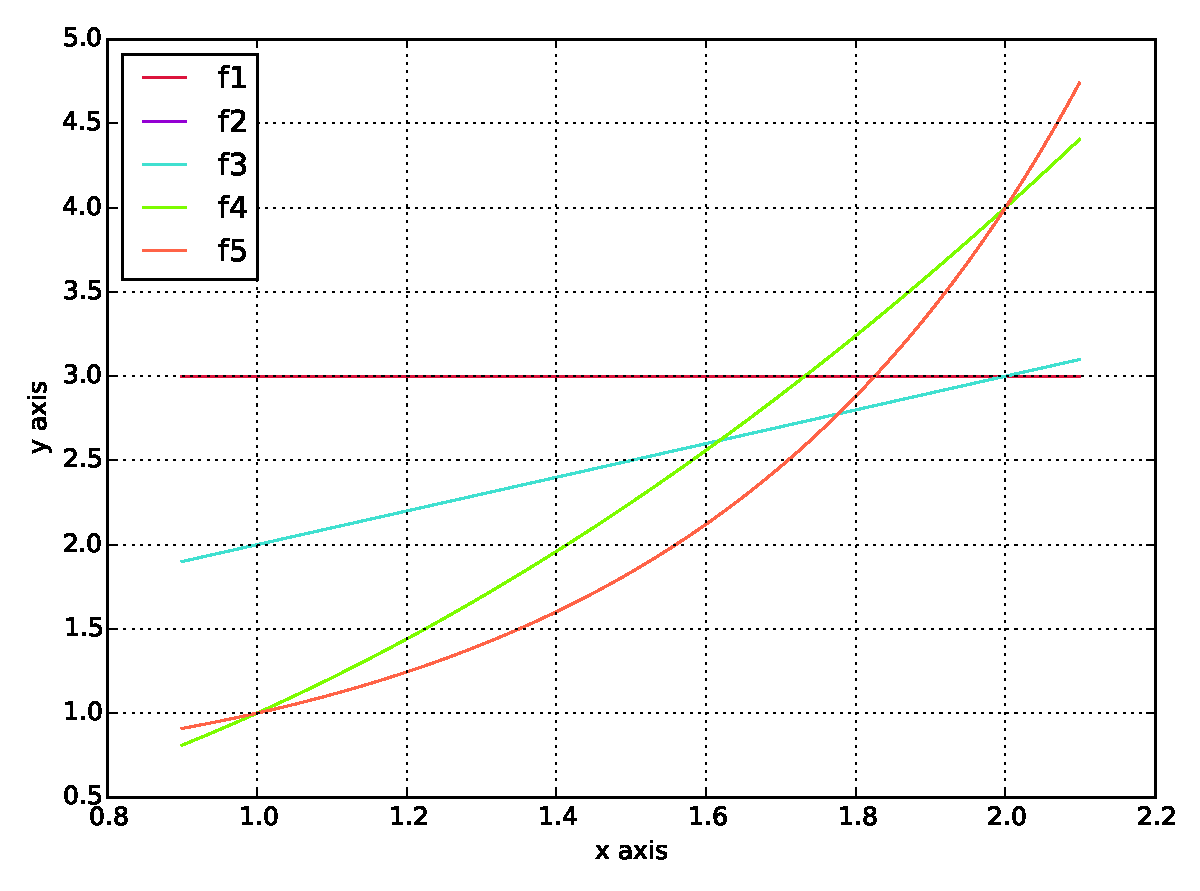
\includegraphics[width=15cm]{171.pdf}


\vspace{1\baselineskip}






\end{document}











